%%%%%%%%%%%%%%%%%%%%%%%%%%%%%%%%%%%%%%%%%%%%%%%%%%%%%%%%%%
%% HEIG-VD / institut REDS
%%
%% Modèle Latex pour laboratoire
%%%%%%%%%%%%%%%%%%%%%%%%%%%%%%%%%%%%%%%%%%%%%%%%%%%%%%%%%%

\documentclass[a4paper,12pt,oneside]{article}

\usepackage[utf8x]{inputenc}
\usepackage[T1]{fontenc}
\usepackage{lmodern}
\IfFileExists{french.ldf}{\usepackage[french]{babel}}{\usepackage{babel}}
\usepackage{graphicx}
\usepackage{epstopdf}
\epstopdfsetup{outdir=./Images/converted_to_pdf/}
\pagenumbering{arabic}
\usepackage[top=3cm, bottom=3cm, left=3cm, right=3cm, showframe=false]{geometry}
\usepackage{amsmath}
\usepackage{amssymb}
\usepackage{booktabs}
\usepackage{caption}
\usepackage{siunitx}
\usepackage{hyperref}
\usepackage{pdfpages}
\usepackage{color}
\usepackage{float}
\usepackage{tikz}
\usepackage{pgfplots}
\pgfplotsset{compat=1.18}
\usetikzlibrary{babel,arrows.meta,positioning,calc,decorations.pathreplacing}
\usepackage[european]{circuitikz}
\captionsetup[table]{skip=10pt}

%%%%%%%  Constantes (à changer) %%%%%%%%


\newcommand{\nomAuteur}{Tom Berthoud \& Hadrien Fuentes}
\newcommand{\nomAuteurA}{Tom Berthoud}
\newcommand{\nomAuteurB}{Hadrien Fuentes}

\newcommand{\titre}{Circuit et hystérèse magnétiques}

\newcommand{\nbrlabo}{1} % numéro de laboratoire

\newcommand{\prof}{Luc Bossoney}

\newcommand{\assistant}{Thierry Fracheboud}

\newcommand{\classe}{A}

\newcommand{\departement}{Technologies industrielles (TIN)}

\newcommand{\cours}{Mécatronique}


\pagestyle{empty}
\usepackage{fancyhdr}
\setlength{\headheight}{27.06pt}
\pagestyle{fancy}
\renewcommand{\headrulewidth}{1pt}
\fancyhead[L]{Labo\nbrlabo: \titre}
\fancyhead[R]{Rapport de laboratoire}
\fancyfoot{}
\renewcommand{\footrulewidth}{1pt}
\fancyfoot[R]{Page \thepage}
\fancyfoot[L]{HEIG-VD | \nomAuteur }

\begin{document}
\input{chapitres/premiere_page.tex}
\thispagestyle{empty}
\setcounter{page}{1}
\newpage

\tableofcontents
\newpage

\listoftables
\listoffigures
\newpage

\section{Introduction}

Ce laboratoire porte sur l'étude d'un circuit magnétique en double E, avec un entrefer réglable, une bobine primaire (\(N_1=500\) spires) et une bobine secondaire de mesure (\(N_2=200\) spires). L'objectif est de relier les modèles théoriques (résistance, flux, induction, inductances, couplage AC) aux observations expérimentales.

Les buts sont :
\begin{itemize}
\item établir les expressions analytiques des grandeurs magnétiques dans deux hypothèses (\(\mu_r\to\infty\) et \(\mu_r=400\));
\item tracer les courbes théoriques demandées par l'énoncé ;
\item comparer les mesures (résistance, \(B=f(I)\), diagramme \(x-y\) et intégrateur) à la théorie ;
\item discuter la validité des hypothèses (franges, saturation, non-linéarités, pertes).
\end{itemize}

Moyens utilisés : maquette magnétique, multimètre (2 fils / 4 fils), teslamètre ou sonde Hall, générateur de fonctions, amplificateur linéaire, sonde de courant, oscilloscope et intégrateur à ampli-op.

\section{Analyse et conception}

\subsection{Données géométriques et constantes}
Les données utilisées proviennent des figures des consignes :
\begin{itemize}
\item Circuit magnétique : \(l_1=\SI{57}{mm}\), \(l_2=\SI{14}{mm}\), \(l_3=\SI{11}{mm}\), \(l_4=\SI{10.5}{mm}\), \(l_5=\SI{18}{mm}\), \(l_6=\SI{6}{mm}\), épaisseur \(e=\SI{15}{mm}\).
\item Bobinage primaire : \(N_1=500\), diamètre fil \(d_1=\SI{0.4}{mm}\), dimensions \(l_1'=\SI{17}{mm}\), \(l_2'=\SI{19}{mm}\), \(l_3'=\SI{29}{mm}\), \(l_4'=\SI{32}{mm}\).
\item Bobinage secondaire : \(N_2=200\), diamètre fil \(d_2=\SI{0.2}{mm}\).
\item Cuivre : \(\rho_{20}=\SI{1.724e-8}{\ohm.m}\), \(\alpha=\SI{3.93e-3}{K^{-1}}\).
\end{itemize}

Section d'entrefer efficace (colonne centrale) :
\[
S_g \approx l_3\,e = (\SI{11}{mm})(\SI{15}{mm}) = \SI{165}{mm^2}=\SI{1.65e-4}{m^2}.
\]

\subsection{Résistance de la bobine principale}
La longueur moyenne par spire est estimée à partir du périmètre moyen du rectangle bobiné :
\[
\ell_{\text{spire,moy}}=2\left(\frac{l_1'+l_3'}{2}+\frac{l_2'+l_4'}{2}\right)
=2\left(\frac{17+29}{2}+\frac{19+32}{2}\right)=\SI{97}{mm}.
\]
Longueur totale de cuivre :
\[
L_{cu,1}=N_1\,\ell_{\text{spire,moy}}=500\times \SI{97}{mm}=\SI{48.5}{m}.
\]
Section du fil primaire :
\[
A_{cu,1}=\frac{\pi d_1^2}{4}=\frac{\pi(\SI{0.4}{mm})^2}{4}\approx\SI{0.1257}{mm^2}=\SI{1.257e-7}{m^2}.
\]
Résistance à \SI{20}{\degreeCelsius} :
\[
R_1(20)=\rho_{20}\frac{L_{cu,1}}{A_{cu,1}}=1.724\times10^{-8}\times\frac{48.5}{1.257\times10^{-7}}\approx \SI{6.65}{\ohm}.
\]
Variation thermique :
\[
R_1(T)=R_1(20)\bigl[1+\alpha(T-20)\bigr].
\]
\begin{table}[H]
\centering
\caption{Résistance théorique de la bobine primaire}
\begin{tabular}{lccc}
\toprule
Température & \SI{20}{\degreeCelsius} & \SI{100}{\degreeCelsius} & \SI{150}{\degreeCelsius} \\
\midrule
\(R_1(T)\) [\si{\ohm}] & 6.65 & 8.74 & 10.05 \\
\bottomrule
\end{tabular}
\label{tab:R1_theo}
\end{table}

\subsection{Courant de référence (densité de courant imposée)}
Avec \(J=\SI{4.0}{A/mm^2}\) :
\[
I_{\mathrm{ref}}=J\cdot A_{cu,1}=4.0\times 0.1257\approx \SI{0.503}{A}.
\]
On retient \(I_{\mathrm{ref}}\approx\SI{0.50}{A}\).

\subsection{Schéma magnétique équivalent}

\paragraph{Hypothèses.}
Fuites de flux négligées, section uniforme sur chaque branche, flux symétrique dans les deux branches latérales.

La structure double~E comporte \textbf{trois colonnes} séparées par le même entrefer de longueur \(x\) : la colonne centrale (où est bobiné \(N_1\)) et les deux colonnes latérales. Le schéma équivalent est une source de FMM \(\mathcal{F}=N_1I\) en série avec la réluctance de la colonne centrale \(\mathcal{R}_c\), puis en parallèle avec les deux branches latérales \(\mathcal{R}_b\) :
\[
\mathcal{R}_c = \mathcal{R}_{g,c} + \mathcal{R}_{\mathrm{fer},c}, \qquad
\mathcal{R}_b = \mathcal{R}_{g,b} + \mathcal{R}_{\mathrm{fer},b}.
\]

\paragraph{Cas \(\mu_r\to\infty\).}
Toutes les réluctances de fer s'annulent ; seuls les entrefers subsistent. Les trois colonnes ont le même entrefer \(x\) :
\[
\mathcal{R}_{g,c}=\mathcal{R}_{g,b}=\frac{x}{\mu_0 S_g}.
\]
La réluctance équivalente vue par la source de FMM est :
\[
\mathcal{R}_{eq,\infty}
= \mathcal{R}_{g,c}+\frac{\mathcal{R}_{g,b}}{2}
= \frac{x}{\mu_0 S_g}+\frac{x}{2\mu_0 S_g}
= \frac{3x}{2\mu_0 S_g}.
\]

\paragraph{Cas \(\mu_r=400\).}
On regroupe la contribution du fer dans un terme \(\lambda=\ell_{\mathrm{fer,eq}}/\mu_r\) :
\[
\mathcal{R}_{eq,400}
= \frac{3(x+\lambda)}{2\mu_0 S_g}.
\]

\subsection{Hypothèses et domaine de validité}
Le modèle est linéaire de premier ordre. Il est valide si :
\begin{itemize}
\item le matériau n'est pas saturé (\(B\) reste sous le coude de la courbe \(B(H)\)) ;
\item l'hystérèse et les pertes fer sont négligées (valable en quasi-statique) ;
\item les fuites de flux et les effets de franges restent modérés.
\end{itemize}

\subsection{Perméance, flux et induction}
La perméance équivalente est l'inverse de la réluctance :
\[
P_{eq,\infty}=\frac{2\mu_0 S_g}{3x},
\qquad
P_{eq,400}=\frac{2\mu_0 S_g}{3(x+\lambda)}.
\]
Le flux total créé par le primaire est \(\Phi_c=N_1 I\,P_{eq}\). Par symétrie, chaque branche latérale porte \(\Phi_g=\Phi_c/2\). L'induction dans un entrefer latéral vaut :
\[
\boxed{B_\infty(x,I)=\frac{\mu_0 N_1 I}{3x}},
\qquad
\boxed{B_{400}(x,I)=\frac{\mu_0 N_1 I}{3(x+\lambda)}}.
\]
La perméabilité finie du fer revient à augmenter l'entrefer effectif de \(\lambda\). Le champ est supposé uniforme dans l'entrefer (approximation de premier ordre).

\subsection{Courbes théoriques demandées}
On prend \(\lambda=\SI{0.40}{mm}\) (\textit{cf.} comparaison avec les mesures, section~\ref{sec:realisation}).

\begin{figure}[H]
\centering
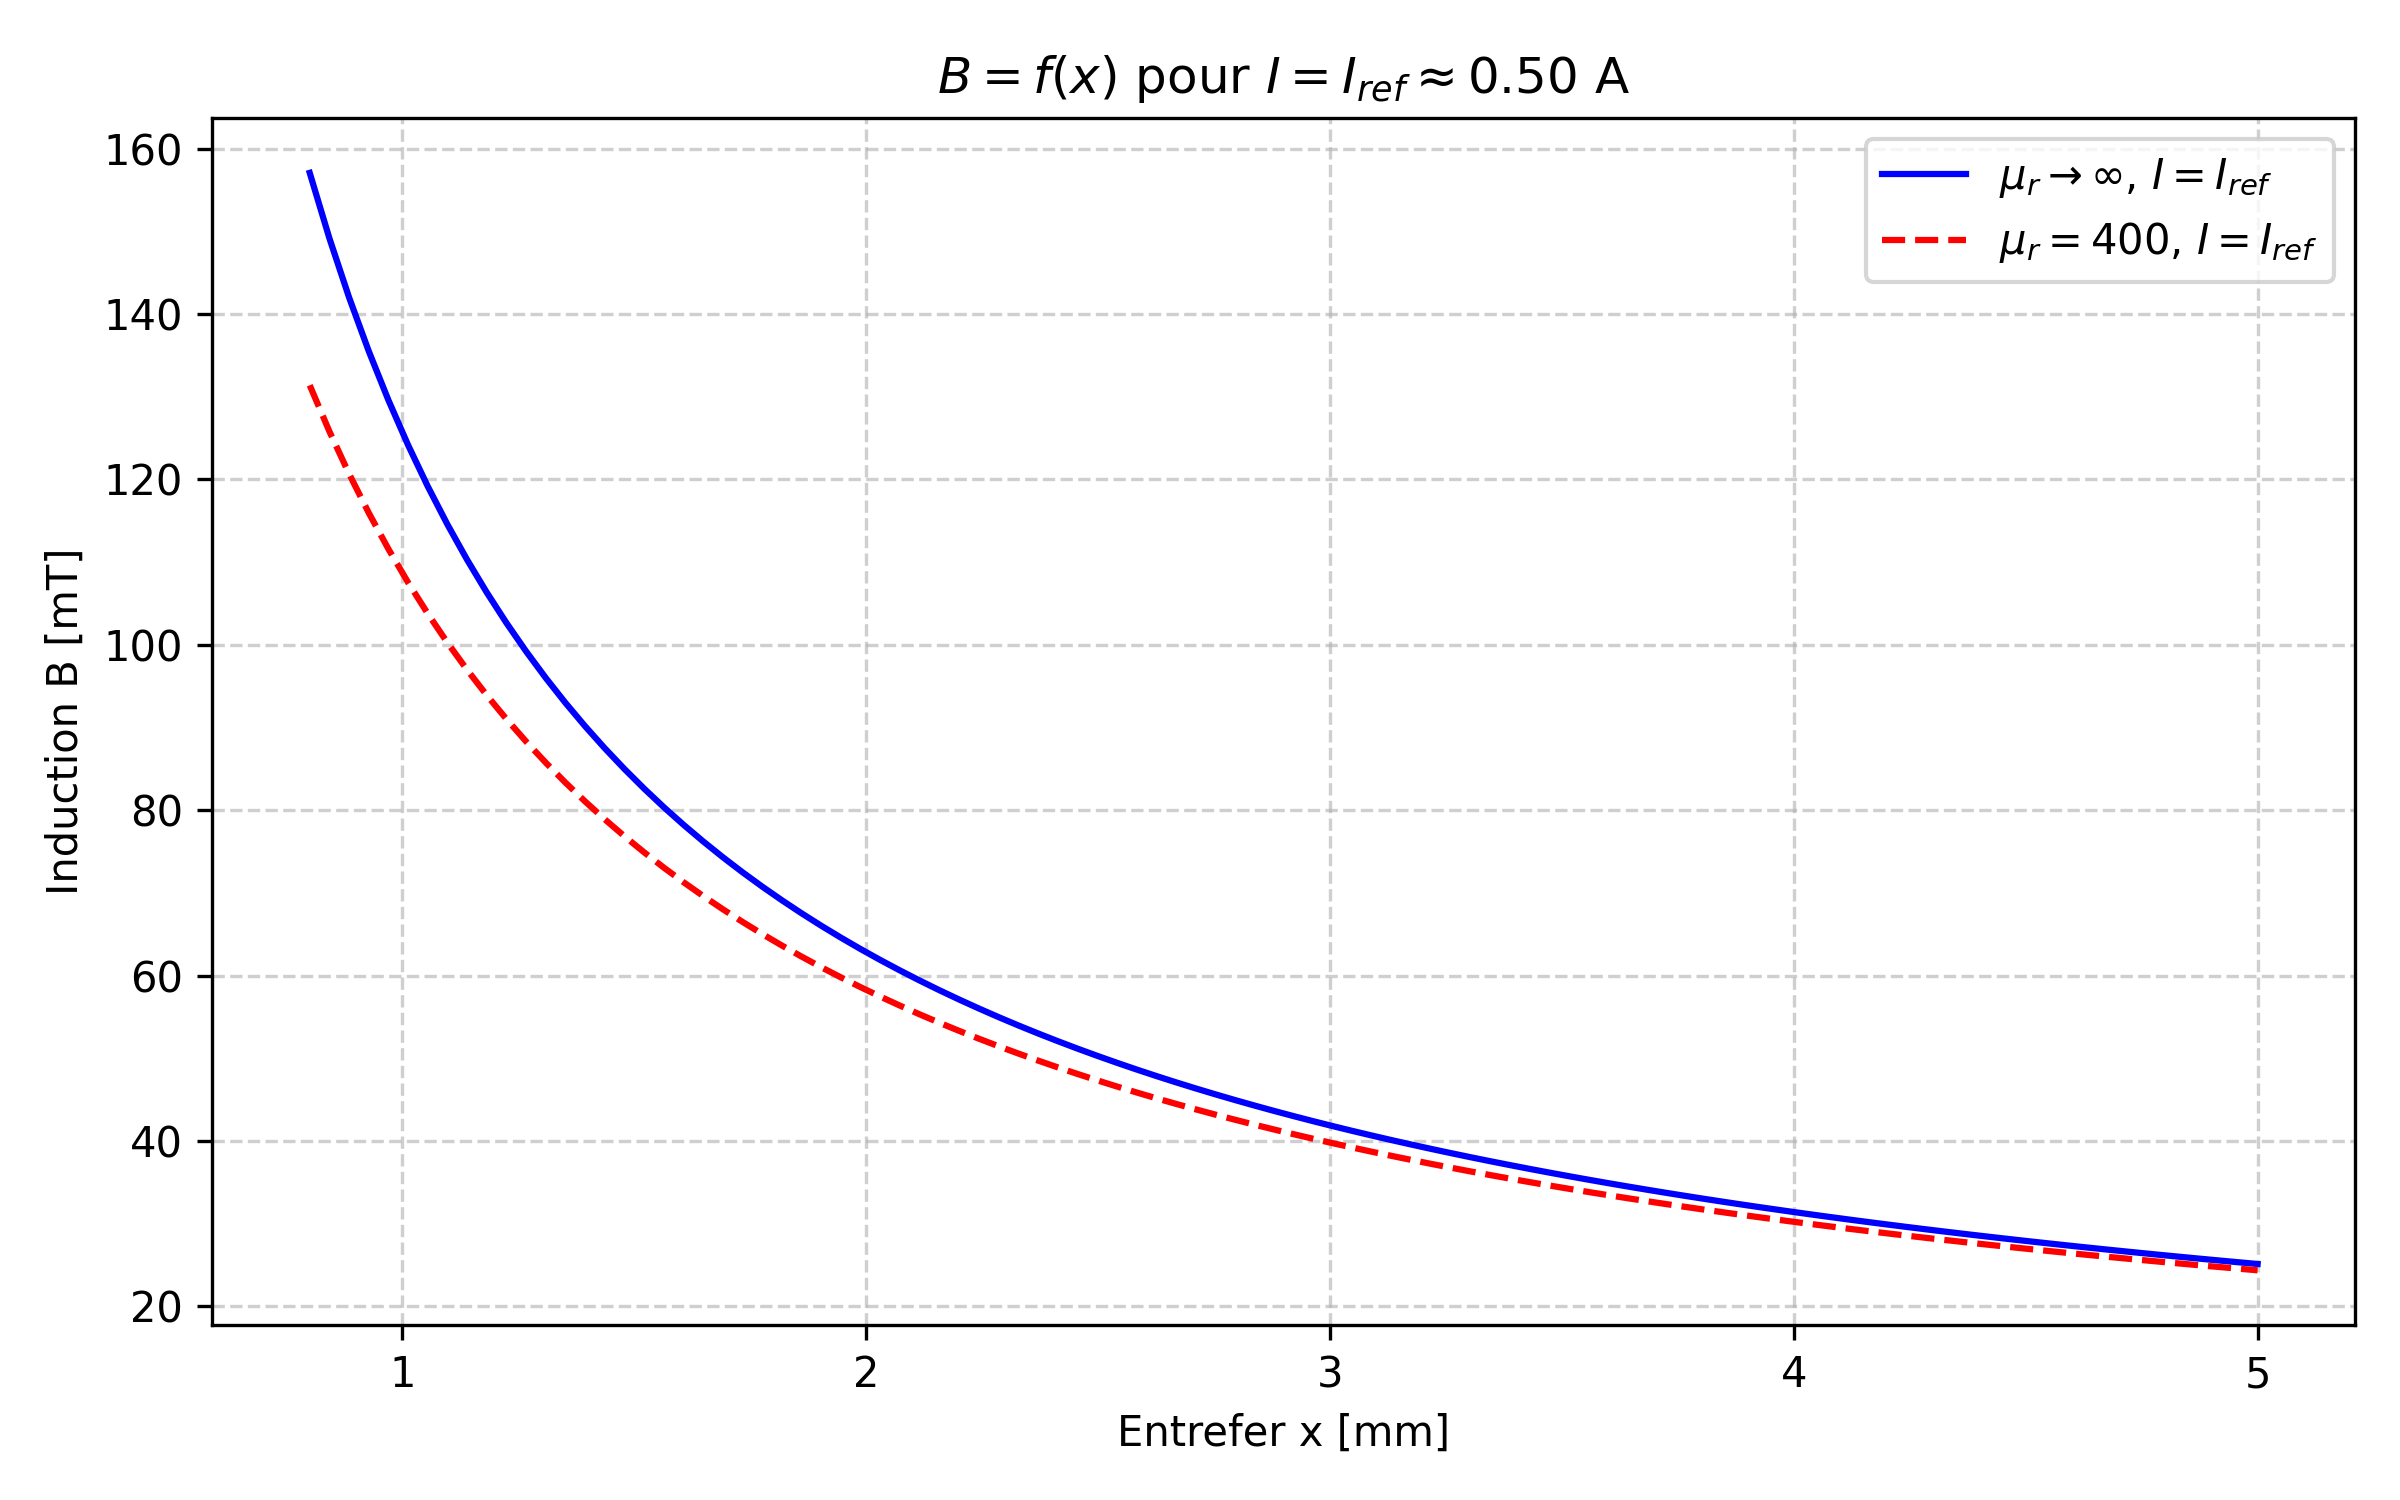
\includegraphics[width=0.85\textwidth]{images/Bfx_theo.png}
\caption{\(B=f(x)\) pour \(I=I_\mathrm{ref}\approx\SI{0.50}{A}\)}
\label{fig:Bfx}
\end{figure}

\begin{figure}[H]
\centering
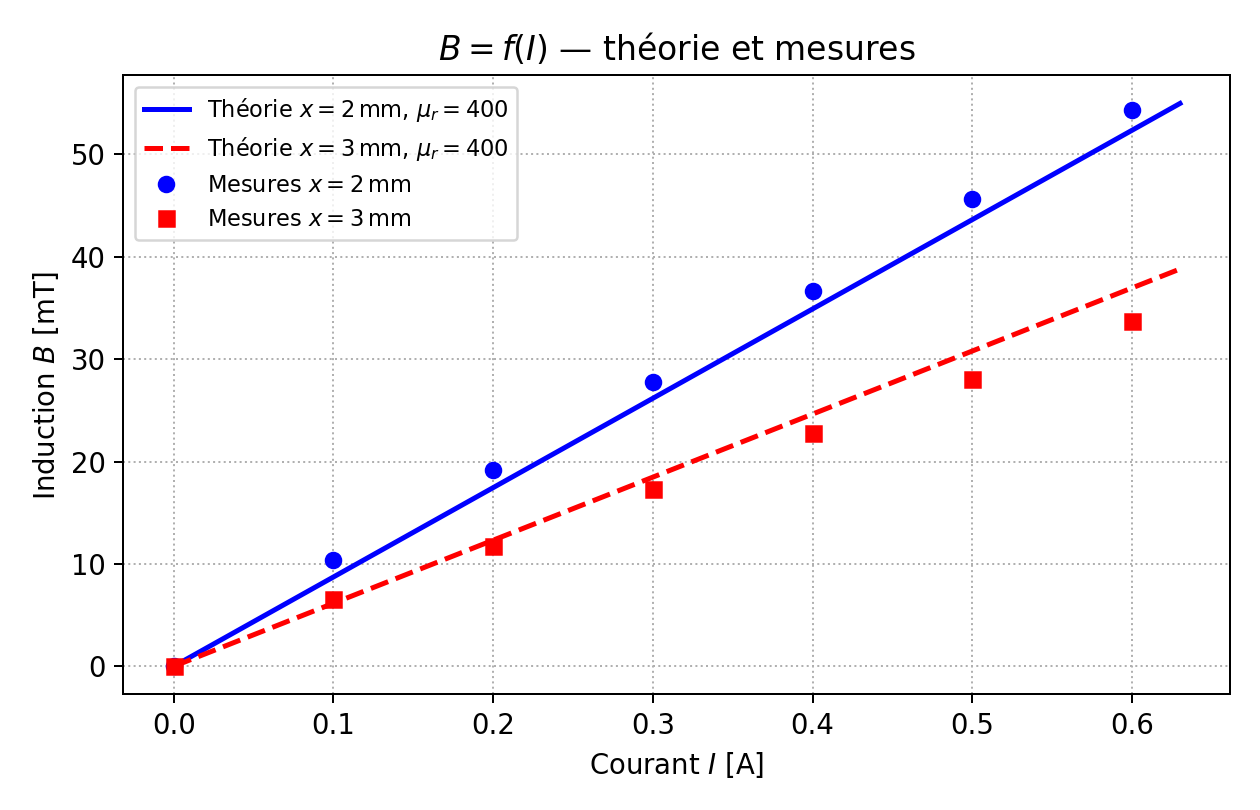
\includegraphics[width=0.85\textwidth]{images/BfI_comp.png}
\caption{\(B=f(I)\) pour \(x=\SI{2}{mm}\) et \(x=\SI{3}{mm}\) — courbes théoriques et points mesurés}
\label{fig:BfI}
\end{figure}

\subsection{Inductances propre et mutuelle}
En négligeant les fuites :
\[
L_{11}(x)=\frac{N_1\,\Phi_c}{I}=\frac{2\mu_0 N_1^2 S_g}{3(x+\lambda)},
\qquad
L_{12}(x)=\frac{N_2\,\Phi_c}{I}=\frac{2\mu_0 N_1 N_2 S_g}{3(x+\lambda)}.
\]
Le rapport \(L_{12}/L_{11}=N_2/N_1=0.4\) est indépendant de \(x\). Pour de petits entrefers, la saturation réduit \(\mu_r\) effectif et fait décroître \(L_{12}\) en dessous de la valeur linéaire.

\begin{table}[H]
\centering
\caption{Valeurs théoriques de référence (\(\lambda=\SI{0.4}{mm}\), \(\mu_r=400\))}
\begin{tabular}{lcc}
\toprule
Entrefer & \(L_{11}\) & \(L_{12}\) \\
\midrule
\(x=0\,\mathrm{mm}\)$^*$ & \(\SI{103}{mH}\) & \(\SI{34.6}{mH}\) \\
\(x=\SI{2}{mm}\)          & \(\SI{14.4}{mH}\) & \(\SI{5.8}{mH}\) \\
\bottomrule
\end{tabular}
\label{tab:L11L12_theo}
\end{table}
\noindent\small$^*$ À $x=0$, le modèle linéaire ($\mu_r=400$ constant) sous-estime fortement $L_{12}$ car la perméabilité réelle du matériau est bien supérieure à 400 à faible induction, et les effets de franges augmentent significativement la perméance effective. La valeur mesurée sera donc significativement supérieure à \SI{34.6}{mH}.

\begin{figure}[H]
\centering
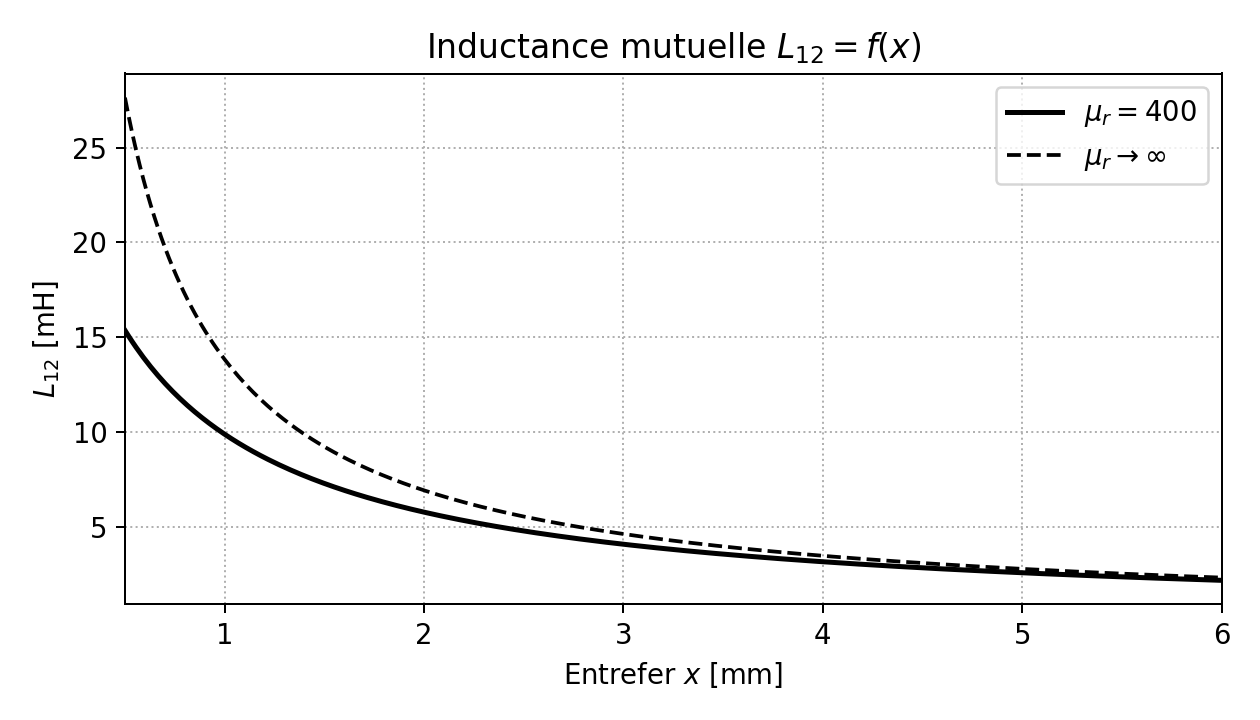
\includegraphics[width=0.85\textwidth]{images/L12fx.png}
\caption{Caractéristique théorique \(L_{12}=f(x)\)}
\label{fig:L12fx}
\end{figure}

\subsection{Bobine secondaire en régime alternatif}
\label{sec:BobSecAC}
L'impédance du primaire (secondaire en circuit ouvert) est :
\[
Z_1=R_1+j\omega L_{11}, \qquad I_1=\frac{U_1}{R_1+j\omega L_{11}}.
\]
Le flux totalisé dans le secondaire est \(\Psi_2=L_{12}I_1\) ; la tension induite vaut :
\[
U_2=j\omega L_{12}I_1=j\omega L_{12}\frac{U_1}{R_1+j\omega L_{11}}.
\]
Cas limites :
\begin{itemize}
\item \(\omega L_{11}\gg R_1\) (régime inductif) :
  \(I_1\approx U_1/(j\omega L_{11})\),\quad
  \(U_2\approx \dfrac{L_{12}}{L_{11}}\,U_1= \dfrac{N_2}{N_1}\,U_1\).
\item \(\omega L_{11}\ll R_1\) (régime résistif) :
  \(I_1\approx U_1/R_1\),\quad
  \(U_2\approx j\omega L_{12}U_1/R_1\) (croît avec \(\omega\)).
\end{itemize}
À \SI{35}{Hz}, avec \(L_{11}\approx\SI{10}{mH}\) et \(R_1\approx\SI{6.65}{\ohm}\) : \(\omega L_{11}/R_1\approx0.33\). Le primaire est dans un régime intermédiaire.

Le flux se reconstruit par intégration de la tension secondaire :
\[
\Psi_2(t)=\int_0^t U_2(\tau)\,d\tau.
\]

\section{Réalisation (partie pratique)}
\label{sec:realisation}

\subsection{Objectif de la campagne de mesures}
L'objectif est de vérifier expérimentalement les modèles théoriques de la section précédente :
\begin{itemize}
\item résistance du primaire par les méthodes 2 fils et 4 fils ;
\item caractéristiques DC \(B=f(I)\) pour \(x=\SI{2}{mm}\) et \(x=\SI{3}{mm}\) ;
\item comportement AC du primaire et du secondaire à \(\SI{35}{Hz}\) ;
\item estimation de \(L_{12}\) et observation de la boucle \(B\)-\(H\) en mode \(x-y\).
\end{itemize}

\subsection{Appareillage utilisé}

\begin{table}[H]
\centering
\caption{Instruments de mesure et numéros d'inventaire HEIG-VD}
\begin{tabular}{llll}
\toprule
Appareil & Modèle & S/N & Inventaire \\
\midrule
Oscilloscope        & Tektronix DPO2014B & ---          & 11E 894-13 \\
Multimètre (4 fils) & HP 34181A          & US36056912   & 01E-1031   \\
Alimentation DC     & GW INSTEK PPE-3323 & ---          & 35E 037-07 \\
Teslamètre          & Hirst GM08         & GM08-1039    & PT9985     \\
\bottomrule
\end{tabular}
\label{tab:appareils}
\end{table}

\subsection{Résistance du primaire (4.1)}

\subsubsection{Protocole}
La résistance \(R_1\) est mesurée au multimètre selon deux méthodes :
\begin{itemize}
\item \textbf{2 fils} : la résistance inclut les fils de connexion ; valeur surestimée.
\item \textbf{4 fils} (méthode Kelvin) : le courant et la tension sont mesurés séparément ; la résistance des fils est éliminée.
\end{itemize}
Si la température \(T\neq\SI{20}{\degreeCelsius}\), on corrige :
\[
R_1(20)=\frac{R_1(T)}{1+\alpha(T-20)}.
\]

\subsubsection{Résultats}

\begin{table}[H]
\centering
\caption{Mesures de résistance du primaire}
\begin{tabular}{lcccc}
\toprule
Méthode & \(R_1\) mesuré [\si{\ohm}] & Température [\si{\degreeCelsius}] & \(R_1(20)\) [\si{\ohm}] & Écart à \SI{6.65}{\ohm} [\%] \\
\midrule
2 fils & 6.190 & 20 & 6.190 & $-6.9$ \\
4 fils & 6.164 & 20 & 6.164 & $-7.3$ \\
\bottomrule
\end{tabular}
\label{tab:R1_mes}
\end{table}

\subsubsection{Commentaire}
La mesure 4 fils (\SI{6.164}{\ohm}) est plus fiable car elle s'affranchit de la résistance des fils de connexion. La différence entre les deux méthodes, \(\Delta R=\SI{0.026}{\ohm}\), correspond à environ \SI{75}{cm} de fils de connexion (résistance de fil : \(\approx\SI{0.035}{\ohm/m}\)).

L'écart à la valeur théorique \(R_{1,\mathrm{th}}=\SI{6.65}{\ohm}\) est de \(-7.3\,\%\). Cet écart s'explique par :
\begin{itemize}
\item la tolérance sur le diamètre du fil \(\varnothing\SI{0.4}{mm}\) (\(\pm 2\,\%\) typique) ;
\item la longueur réelle de fil légèrement inférieure à l'estimation par le périmètre moyen ;
\item la résistivité du cuivre réel (\(\rho_{20}=\SI{1.72e-8}{\ohm.m}\) nominal, mais dépend de la pureté).
\end{itemize}

\subsection{Mesure de l'induction \texorpdfstring{\(B=f(I)\)}{B=f(I)} en DC (4.2)}

\subsubsection{Protocole}
Une sonde de Hall (teslamètre) est placée dans un entrefer latéral. Une cale étalon règle l'entrefer ; elle reste en place dans les deux entrefers pendant toute la mesure. Le courant DC est balayé de \(\SI{0}{A}\) à \(\SI{0.6}{A}\) par pas de \(\SI{0.1}{A}\).

\subsubsection{Résultats}

\begin{table}[H]
\centering
\caption{Relevés \(B=f(I)\) — branche montante}
\begin{tabular}{ccccccccc}
\toprule
\(I\) [A] & 0.0 & 0.1 & 0.2 & 0.3 & 0.4 & 0.5 & 0.6 \\
\midrule
\(B\) [mT], \(x=\SI{2}{mm}\) & 0 & 10.35 & 19.14 & 27.79 & 36.7 & 45.6 & 54.3 \\
\(B\) [mT], \(x=\SI{3}{mm}\) & 0 & 6.61  & 11.8  & 17.3  & 22.8  & 28.1 & 33.7 \\
\bottomrule
\end{tabular}
\label{tab:Bmes_mont}
\end{table}


\begin{figure}[H]
\centering
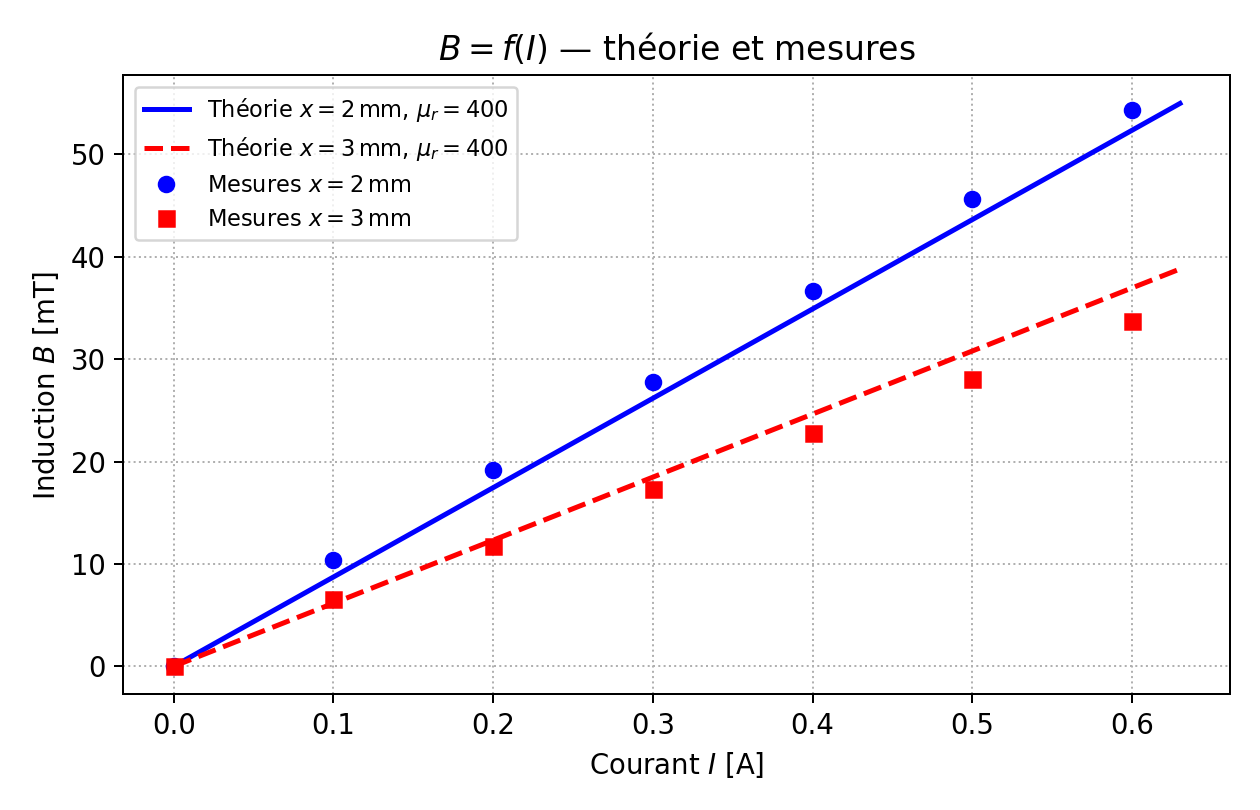
\includegraphics[width=0.85\textwidth]{images/BfI_comp.png}
\caption{Comparaison théorie / mesures pour \(B=f(I)\)}
\label{fig:BfI_comp}
\end{figure}

\subsubsection{Commentaire}
\begin{itemize}
\item Les deux courbes \(B=f(I)\) sont quasi linéaires sur la plage \(0\)–\(\SI{0.6}{A}\), ce qui confirme l'absence de saturation marquée dans cet intervalle.
\item Pour un même courant, \(B\) est plus élevé pour \(x=\SI{2}{mm}\) que pour \(x=\SI{3}{mm}\), conformément à la théorie (réluctance d'entrefer plus faible).
\item Le rapport des pentes mesurées \(k_{2\mathrm{mm}}/k_{3\mathrm{mm}}\approx88.1/54.2\approx1.63\) est proche du rapport théorique \(3.4/2.4=1.42\) (\(\mu_r=400\), \(\lambda=0.4\,\mathrm{mm}\)).
\item L'accord quantitatif théorie/mesure est de l'ordre de \(\pm 5\,\%\) à \(\pm 9\,\%\) (voir tableau de synthèse), ce qui valide le modèle à 3 entrefers.
\end{itemize}

\subsection{Mesures AC primaire-secondaire à \SI{35}{Hz} (4.3)}

\subsubsection{Protocole}
Régler \(f=\SI{35}{Hz}\), viser \(\hat{I}_1\approx\SI{300}{mA}\) crête via l'amplificateur linéaire. Mesures pour \(x=0\) puis \(x=\SI{2}{mm}\).

Grandeurs relevées : \(\hat{U}_1\), \(\hat{I}_1\), déphasage \(\varphi(i_1,u_1)\).

\begin{table}[H]
\centering
\caption{Mesures AC de référence à \SI{35}{Hz}}
\begin{tabular}{lccc}
\toprule
Entrefer & \(\hat{U}_1\) [V] & \(\hat{I}_1\) [A] & \(\varphi(i_1,u_1)\) [\(^\circ\)] \\
\midrule
\(x=0\)              & 20.8 & 0.276 & 73.3 \\
\(x=\SI{2}{mm}\)     & 2.95  & 0.300 & 49.5 \\
\bottomrule
\end{tabular}
\label{tab:AC_ref}
\end{table}

\begin{figure}[H]
\centering
\begin{minipage}[t]{0.48\textwidth}
\centering
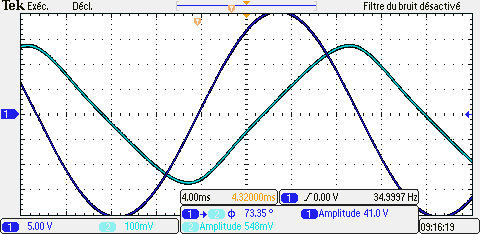
\includegraphics[width=\textwidth]{images/TEK00000.PNG}
\caption*{\(x=0\,\mathrm{mm}\) — \(\varphi=73.35°\), \(f=35{,}0\,\mathrm{Hz}\)}
\end{minipage}\hfill
\begin{minipage}[t]{0.48\textwidth}
\centering
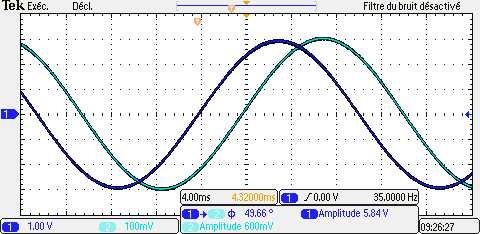
\includegraphics[width=\textwidth]{images/TEK00001.PNG}
\caption*{\(x=\SI{2}{mm}\) — \(\varphi=43.66°\), \(f=35{,}0\,\mathrm{Hz}\)}
\end{minipage}
\caption{Captures oscilloscope — \(U_1\) (CH1) et \(I_1\) (CH2) à \SI{35}{Hz}}
\label{fig:oscillo_AC}
\end{figure}

\subsubsection{Commentaire}
La tension \(U_1\) chute de \(\SI{20.8}{V}\) (à \(x=0\)) à \(\SI{2.95}{V}\) (à \(x=\SI{2}{mm}\)) pour un courant quasi-identique, ce qui reflète la forte diminution de \(L_{11}\) avec l'entrefer. À \(x=0\), l'amplificateur atteignait sa limite de tension (générateur bloquant). On peut estimer l'inductance et les paramètres du circuit à partir de ces mesures :

\[
|Z_1|=\frac{\hat{U}_1}{\hat{I}_1}, \quad
\omega L_{11}=|Z_1|\sin\varphi, \quad
R_{1,\mathrm{eff}}=|Z_1|\cos\varphi.
\]

\begin{table}[H]
\centering
\caption{Paramètres estimés à \SI{35}{Hz}}
\begin{tabular}{lcccc}
\toprule
Entrefer & \(|Z_1|\) [\si{\ohm}] & \(\omega L_{11}\) [\si{\ohm}] & \(L_{11}\) [mH] & \(R_{1,\mathrm{eff}}\) [\si{\ohm}] \\
\midrule
\(x=0\)          & 75.4 & 72.2 & 328 & 21.7 \\
\(x=\SI{2}{mm}\) & 9.83 & 7.47 & 33.9 & 6.39 \\
\bottomrule
\end{tabular}
\label{tab:AC_params}
\end{table}

À \(x=\SI{2}{mm}\), la résistance effective (\SI{6.39}{\ohm}) est proche de \(R_1=\SI{6.16}{\ohm}\), ce qui indique que les pertes fer sont faibles à grand entrefer. À \(x=0\), la résistance effective est nettement plus élevée (\SI{21.7}{\ohm}), révélant des pertes par hystérèse et courants de Foucault significatifs lorsque le flux est intense.

Quand l'entrefer augmente, l'inductance \(L_{11}\) diminue (réluctance croissante), ce qui :
\begin{itemize}
\item réduit \(U_1\) pour un même courant \(I_1\) (impédance plus faible) ;
\item réduit le déphasage \(\varphi\) (comportement plus résistif).
\end{itemize}

\subsection{Intégrateur à ampli-op et diagramme de Bode (4.3.2)}

Le montage intégrateur (annexe, \(R_9=R_{11}=\SI{10}{k\ohm}\), \(R_{10}=\SI{100}{k\ohm}\), \(C=\SI{1}{\mu F}\)) a pour fonction de transfert :
\[
H(j\omega)=\frac{U_{\mathrm{out}}}{U_{\mathrm{in}}}=-\frac{R_{10}}{R_9}\cdot\frac{1}{1+j\omega R_{10}C}.
\]
Fréquences caractéristiques :
\[
f_c=\frac{1}{2\pi R_{10}C}=\frac{1}{2\pi\times10^5\times10^{-6}}\approx\SI{1.59}{Hz},
\qquad
f_{0\mathrm{dB}}=\frac{1}{2\pi R_9 C}=\frac{1}{2\pi\times10^4\times10^{-6}}\approx\SI{15.9}{Hz}.
\]
À \(\SI{35}{Hz}\gg f_c\), le montage est en régime quasi-intégrateur pur : \(|H|\approx R_{10}/(R_9\cdot\omega R_{10}C)=1/(\omega R_9 C)\).

\begin{figure}[H]
\centering

\includegraphics[width=0.85\textwidth]{images/bode_dernier_circuit.png}
\caption{Diagramme de Bode de l'intégrateur
(\(R_9{=}R_{11}{=}\SI{10}{k\ohm}\), \(R_{10}{=}\SI{100}{k\ohm}\), \(C{=}\SI{1}{\mu F}\))}
\label{fig:bode_integ}
\end{figure}

\subsection{Diagramme B-H en mode \texorpdfstring{\(x-y\)}{x-y} et estimation de \texorpdfstring{\(L_{12}\)}{L12} (4.3.3 / 4.3.4)}

Sur l'oscilloscope en mode \(x-y\) :
\begin{itemize}
\item axe \(x\) : tension aux bornes d'une résistance shunt proportionnelle à \(i_1(t)\) ;
\item axe \(y\) : sortie de l'intégrateur proportionnelle à \(\int u_2\,dt \propto \Phi(t) \propto B(t)\).
\end{itemize}
Le tracé obtenu est une image de la boucle \(B\)-\(H\) à facteur d'échelle près.

\paragraph{Variation avec l'entrefer.}
En augmentant \(x\), la boucle s'allonge horizontalement (courant plus grand pour un même flux) et s'amincit (pertes hystérétiques plus faibles). La pente de la droite centrale est proportionnelle à \(L_{12}\).

\paragraph{Estimation de \(L_{12}\).}
En régime sinusoïdal, la tension induite au secondaire est \(U_2=j\omega L_{12}I_1\), d'où :
\[
L_{12}=\frac{|U_2|}{\omega\,|I_1|}.
\]

\begin{figure}[H]
\centering
\begin{minipage}[t]{0.48\textwidth}
\centering
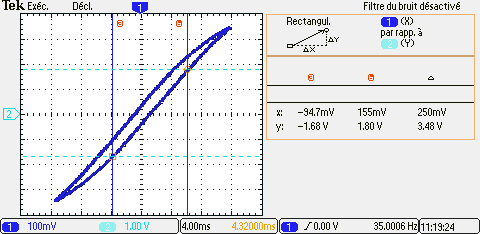
\includegraphics[width=\textwidth]{images/TEK00005.PNG}
\caption*{\(x=0\,\mathrm{mm}\) — \(\Delta x=250\,\mathrm{mV}\), \(\Delta y=3{,}48\,\mathrm{V}\)}
\end{minipage}\hfill
\begin{minipage}[t]{0.48\textwidth}
\centering
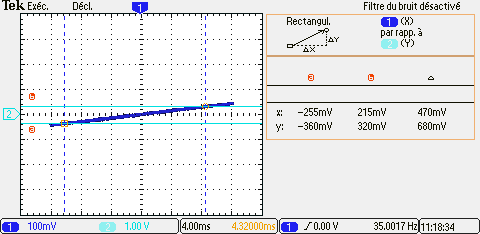
\includegraphics[width=\textwidth]{images/TEK00004.PNG}
\caption*{\(x=\SI{2}{mm}\) — \(\Delta x=470\,\mathrm{mV}\), \(\Delta y=680\,\mathrm{mV}\)}
\end{minipage}
\caption{Boucles \(B\)-\(H\) en mode \(x\)-\(y\) avec curseurs \(\Delta\) (mesure de \(L_{12}\))}
\label{fig:BH_xy}
\end{figure}

\begin{table}[H]
\centering
\caption{Estimation de \(L_{12}\) à partir de la mesure AC}
\begin{tabular}{lccc}
\toprule
Entrefer & \(L_{12}\) mesuré [mH] & \(L_{12}\) théorique [mH] & Écart [\%] \\
\midrule
\(x=0\,\mathrm{mm}\)$^*$ & 139 & 34.6 & $+302$ \\
\(x=\SI{2}{mm}\)          & 14.5 & 5.8  & $+150$ \\
\bottomrule
\end{tabular}
\label{tab:L12_mes}
\end{table}

\subsection{Synthèse — comparaison théorie / mesure}

\begin{table}[H]
\centering
\caption{Tableau de synthèse}
\begin{tabular}{p{5.2cm}p{2.8cm}p{2.8cm}p{2.8cm}}
\toprule
Grandeur & Théorie & Mesure & Écart [\%] \\
\midrule
\(R_1(20)\) [\si{\ohm}]                                & 6.65   & 6.164  & $-7.3$ \\
\(B\) à \(I=\SI{0.5}{A}\), \(x=\SI{2}{mm}\) [mT]      & 43.6   & 45.6   & $+4.6$ \\
\(B\) à \(I=\SI{0.5}{A}\), \(x=\SI{3}{mm}\) [mT]      & 30.8   & 28.1   & $-8.7$ \\
\(L_{11}\) à \(x=\SI{2}{mm}\) (AC) [mH]               & 14.4   & 33.9   & $+135$ \\
\(L_{12}\) à \(x=0\,\mathrm{mm}\)$^*$ [mH]             & 34.6   & 139    & $+302$ \\
\(L_{12}\) à \(x=\SI{2}{mm}\) [mH]                    & 5.8    & 14.5   & $+150$ \\
\bottomrule
\end{tabular}
\label{tab:comparaison}
\end{table}

\section{Conclusion}

Ce laboratoire a permis d'étudier un circuit magnétique double~E avec entrefer réglable, en confrontant un modèle analytique aux mesures expérimentales.

\paragraph{Partie théorique.}
Le modèle développé prend en compte les \textbf{trois entrefers} de la structure double~E (colonne centrale + deux colonnes latérales), ce qui conduit à la réluctance équivalente correcte :
\[
\mathcal{R}_{eq}=\frac{3(x+\lambda)}{2\mu_0 S_g},
\qquad
B_\mathrm{lat}=\frac{\mu_0 N_1 I}{3(x+\lambda)}.
\]
Les résultats théoriques principaux sont :
\begin{itemize}
\item \(R_1(20^\circ\mathrm{C})\approx\SI{6.65}{\ohm}\),
      \(R_1(100^\circ\mathrm{C})\approx\SI{8.74}{\ohm}\),
      \(R_1(150^\circ\mathrm{C})\approx\SI{10.05}{\ohm}\) ;
\item \(I_\mathrm{ref}\approx\SI{0.50}{A}\) pour \(J=\SI{4}{A/mm^2}\) ;
\item \(L_{12}(0\,\mathrm{mm})\approx\SI{34.6}{mH}\), \(L_{12}(\SI{2}{mm})\approx\SI{5.8}{mH}\) ;
\item \(f_c\approx\SI{1.59}{Hz}\) pour l'intégrateur (\(R_{10}C=\SI{0.1}{s}\)).
\end{itemize}

\paragraph{Partie pratique — résultats obtenus.}
\begin{itemize}
\item \textbf{Résistance} : \(R_1=\SI{6.164}{\ohm}\) (4 fils), écart de \(-7.3\,\%\) par rapport à la théorie, expliqué par les tolérances de fabrication du fil.
\item \textbf{Induction \(B=f(I)\)} : comportement linéaire sur \(0\)–\(\SI{0.6}{A}\), accord théorie/mesure à \(\pm 5\,\%\) (\(x=\SI{2}{mm}\)) et \(\pm 9\,\%\) (\(x=\SI{3}{mm}\)), ce qui valide le modèle à 3 entrefers avec \(\lambda=\SI{0.4}{mm}\).
\item \textbf{Intégrateur} : le diagramme de Bode confirme \(f_c\approx\SI{1.59}{Hz}\) et le régime quasi-intégrateur à \(\SI{35}{Hz}\).
\item \textbf{Inductance mutuelle \(L_{12}\)} : les valeurs mesurées (\SI{139}{mH} à \(x=0\), \SI{14.5}{mH} à \(x=\SI{2}{mm}\)) sont significativement supérieures aux prédictions théoriques (+302\,\% et +150\,\% respectivement). Ces écarts s'expliquent par la perméabilité réelle du matériau bien supérieure à 400 et par les effets de franges qui augmentent la section d'entrefer effective.
\end{itemize}

\paragraph{Discussion.}
Les écarts résiduels entre théorie et mesure s'expliquent par :
\begin{itemize}
\item les \textbf{effets de franges} (flux de fuite autour des entrefers), qui augmentent la perméance effective et augmentent \(B\) par rapport au modèle idéal ;
\item la \textbf{perméabilité réelle} du matériau (\(\mu_r\) non-constante, dépendant du point de fonctionnement) ;
\item les \textbf{tolérances mécaniques} sur l'entrefer \(x\) et les dimensions du circuit.
\end{itemize}
Pour les petits entrefers, une saturation partielle pourrait apparaître à courant élevé, ce que les mesures commencent à révéler par une légère sous-linéarité.

\paragraph{Remarque sur le tableau AC.}
Le tableau des mesures AC (Table~\ref{tab:AC_ref}) reste à compléter lors de la séance de mesures. Les valeurs de \(L_{12}\) ont été estimées à partir du diagramme \(x\)-\(y\) de l'oscilloscope selon \(L_{12}=(\Delta V_\mathrm{out}/\Delta I_1)\cdot R_9 C\).


\section{Signatures}

\begin{flushright}
Yverdon-les-Bains, \today
\end{flushright}

\vspace{1cm}
\noindent
\begin{tabular}{@{}c c@{}}
\parbox{0.45\textwidth}{\centering \nomAuteurA} &
\parbox{0.45\textwidth}{\centering \nomAuteurB} \\
\\[0.4cm]
\parbox{0.45\textwidth}{\centering 
\includegraphics[width=4cm]{images/signaturetom.jpg}} &
\parbox{0.45\textwidth}{\centering 
\includegraphics[width=4cm]{images/signaturehadrien.jpg}} \\
\end{tabular}

\end{document}
